\documentclass[10pt,a4paper]{article}
\usepackage[T1]{fontenc}
\usepackage[utf8]{inputenc}
\usepackage[margin=22mm]{geometry}
\usepackage{graphicx}
\usepackage{booktabs}
\usepackage{amsmath}
\usepackage{float}
\usepackage[hidelinks]{hyperref}
\usepackage[font=small,labelfont=bf]{caption}
\setlength{\parindent}{0pt}
\setlength{\parskip}{5pt}
\setlength{\textfloatsep}{12pt}
\setlength{\intextsep}{10pt}
\renewcommand{\arraystretch}{1.15}
\graphicspath{{figures/}}
\raggedbottom

\title{\vspace{-1.5cm}Classifying Stars, Galaxies and Quasars\\
using SDSS Photometry}
% Add your name between the braces below.
\author{}
\date{October 2026}

\begin{document}
\maketitle
\vspace{-1.2cm}

\begin{abstract}
This project explores whether basic machine-learning models can classify
astronomical objects using photometric measurements. A sample of 50,000 objects
was prepared with SQL and analysed in Python. A Random Forest gave the best
test performance, with 95.00\% accuracy and a macro F1-score of 0.911.
Quasars were the most difficult class to identify, and performance was lower
for fainter objects. Removing measurement-uncertainty features reduced accuracy
to 93.11\%. The project demonstrates a repeatable workflow from a raw catalogue
to model comparison and error analysis.
\end{abstract}

\section{Aim}
The aim was to learn how to prepare data, compare classification models and
interpret their errors using an astronomical dataset. The question was:
\emph{how well can photometric measurements predict whether an object is a
star, galaxy or quasar?}
The labels come from SDSS spectroscopy, so the models learn to predict those
catalogue labels. Spectroscopic redshift is excluded from the inputs to keep
the task based on photometry.

\section{Data and features}
The input is a 50,000-object SDSS export, described in the original project
notes as a DR17 SpecPhoto sample~\cite{sdss}. It contains 29,036 galaxies
(58.07\%), 16,326 stars (32.65\%) and 4,638 quasars (9.28\%). The class
labels are \texttt{GALAXY}, \texttt{STAR} and \texttt{QSO}.

SQL was used through DuckDB to prepare the data and calculate four colour
indices. The 14 model inputs are:
\begin{itemize}\setlength{\itemsep}{0pt}
  \item five model magnitudes: $u$, $g$, $r$, $i$ and $z$;
  \item four colours: $u-g$, $g-r$, $r-i$ and $i-z$;
  \item the measurement uncertainty in each of the five magnitudes.
\end{itemize}
A colour is the difference between two magnitudes. The $z$-band magnitude
is a photometric measurement and is distinct from spectroscopic redshift.
Data checks required unique object IDs, recognised labels, finite positive
magnitudes and finite nonnegative uncertainties. All 50,000 rows passed.

\begin{figure}[H]
  \centering
  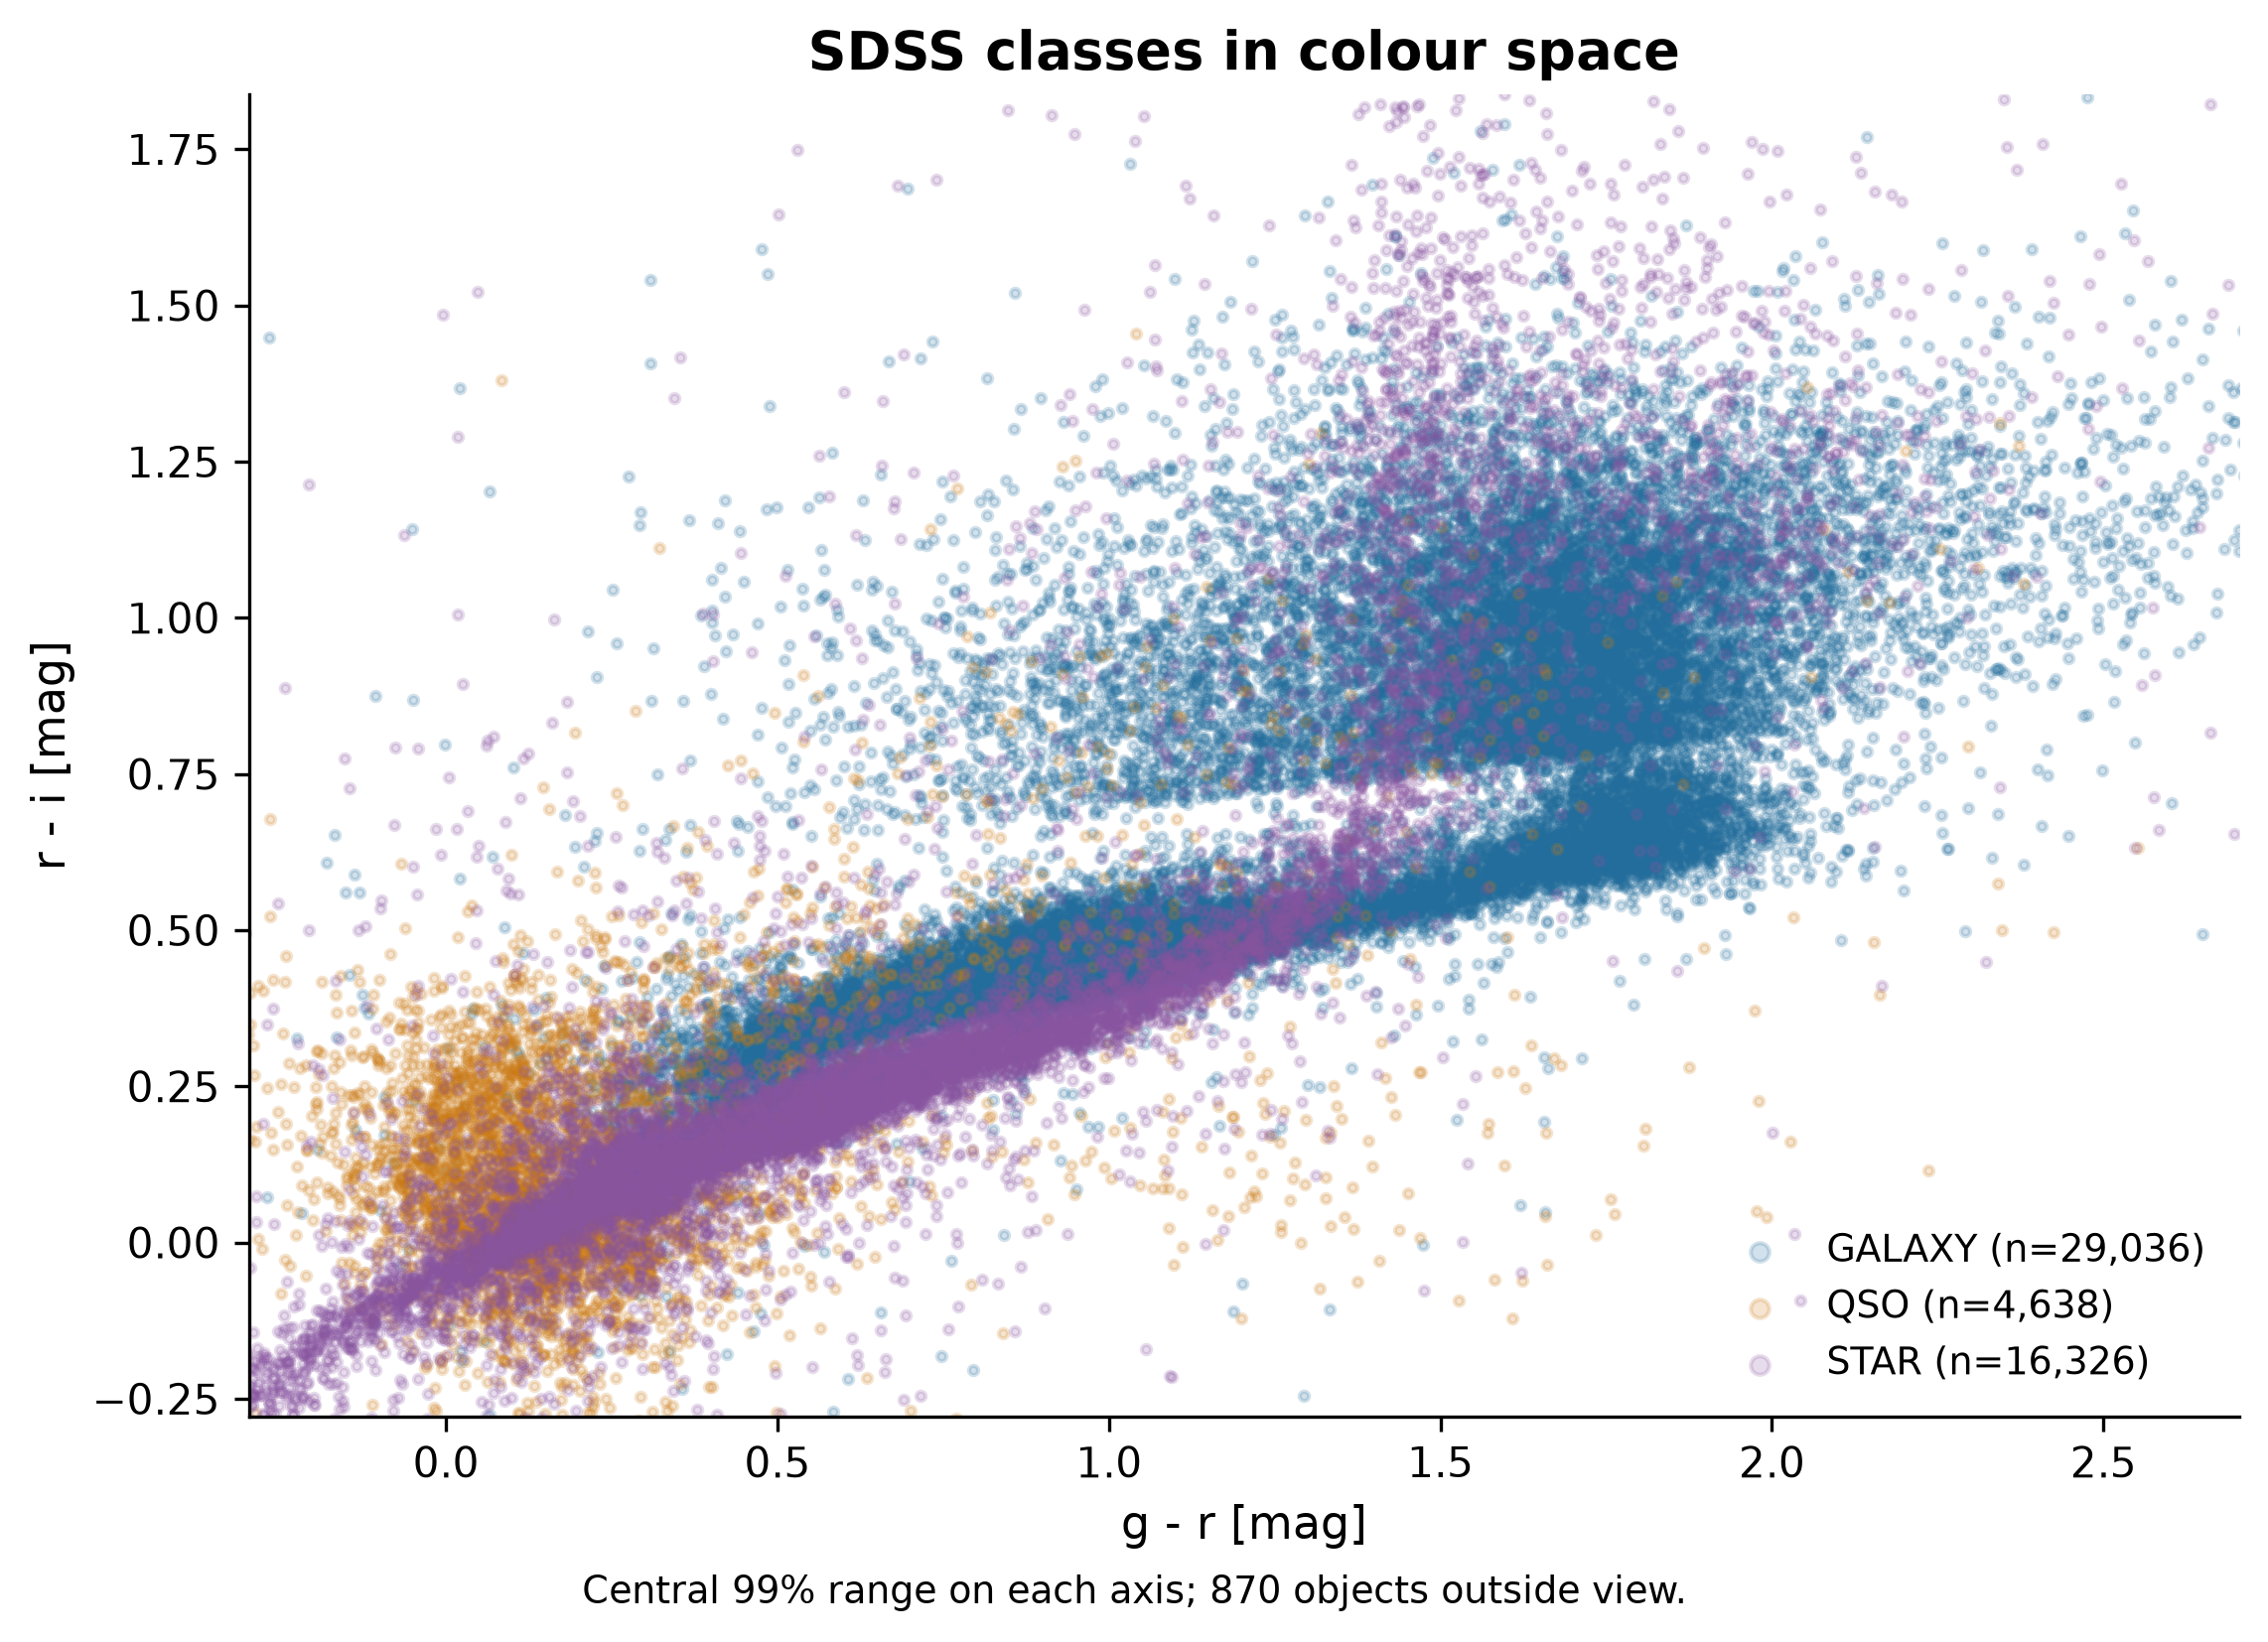
\includegraphics[width=0.66\textwidth]{colour_colour_diagram.png}
  \caption{The classes occupy partly overlapping regions of colour space.
  The plot shows the central 99\% range on each axis; 870 objects lie outside
  the displayed area but remain in the analysis.}
  \label{fig:colours}
\end{figure}

\section{Method}
The data were split into 40,000 training objects and 10,000 test objects.
The split preserved approximately the same class proportions in both sets
and used random seed 42. Every model used the same split.

Four approaches were compared using scikit-learn~\cite{sklearn}:
\begin{itemize}\setlength{\itemsep}{0pt}
  \item a \textbf{majority baseline}, which always predicts the most common
  training class, GALAXY;
  \item \textbf{logistic regression}, a linear classifier, with features
  standardised using the training data;
  \item a \textbf{decision tree}, limited to a maximum depth of 10;
  \item a \textbf{Random Forest}, which combines predictions from many trees.
\end{itemize}
Five-fold stratified cross-validation was applied within the training set:
the model was repeatedly fitted on four parts and checked on the remaining
part. Standardisation was fitted separately within each fold.
The forest used 200 trees and no maximum depth. Minimum leaf sizes of
1, 2, 4, 8 and 16 were compared; size 1 had the highest mean validation
accuracy, 95.06\%. Test results were calculated after this selection.

\section{Model performance}
Accuracy measures the fraction of correctly classified objects. Because the
classes are unequal in size, macro F1 is also reported: it averages each
class's F1-score equally. F1 combines precision and recall.

\begin{table}[H]
  \centering
  \caption{Performance on the same 10,000 test objects. The final row removes
  the five uncertainty features while keeping the forest settings fixed.}
  \label{tab:models}
  \begin{tabular}{lrr}
    \toprule
    Model & Accuracy (\%) & Macro F1 \\
    \midrule
    Majority baseline & 58.07 & 0.245 \\
    Logistic regression & 77.71 & 0.721 \\
    Decision tree & 92.81 & 0.880 \\
    Random Forest & \textbf{95.00} & \textbf{0.911} \\
    Random Forest without uncertainties & 93.11 & 0.893 \\
    \bottomrule
  \end{tabular}
\end{table}

The Random Forest correctly classified 9,500 objects. Its improvement over
logistic regression suggests that nonlinear patterns help distinguish the
classes in this dataset.

\begin{table}[H]
  \centering
  \caption{Random Forest results by class. Precision is the fraction of
  predictions for a class that are correct; recall is the fraction of actual
  members of that class recovered by the model.}
  \label{tab:classes}
  \begin{tabular}{lrrrr}
    \toprule
    Class & Precision & Recall & F1 & Test objects \\
    \midrule
    GALAXY & 0.971 & 0.984 & 0.978 & 5,807 \\
    QSO & 0.834 & 0.798 & 0.816 & 928 \\
    STAR & 0.943 & 0.933 & 0.938 & 3,265 \\
    \bottomrule
  \end{tabular}
\end{table}

\begin{figure}[H]
  \centering
  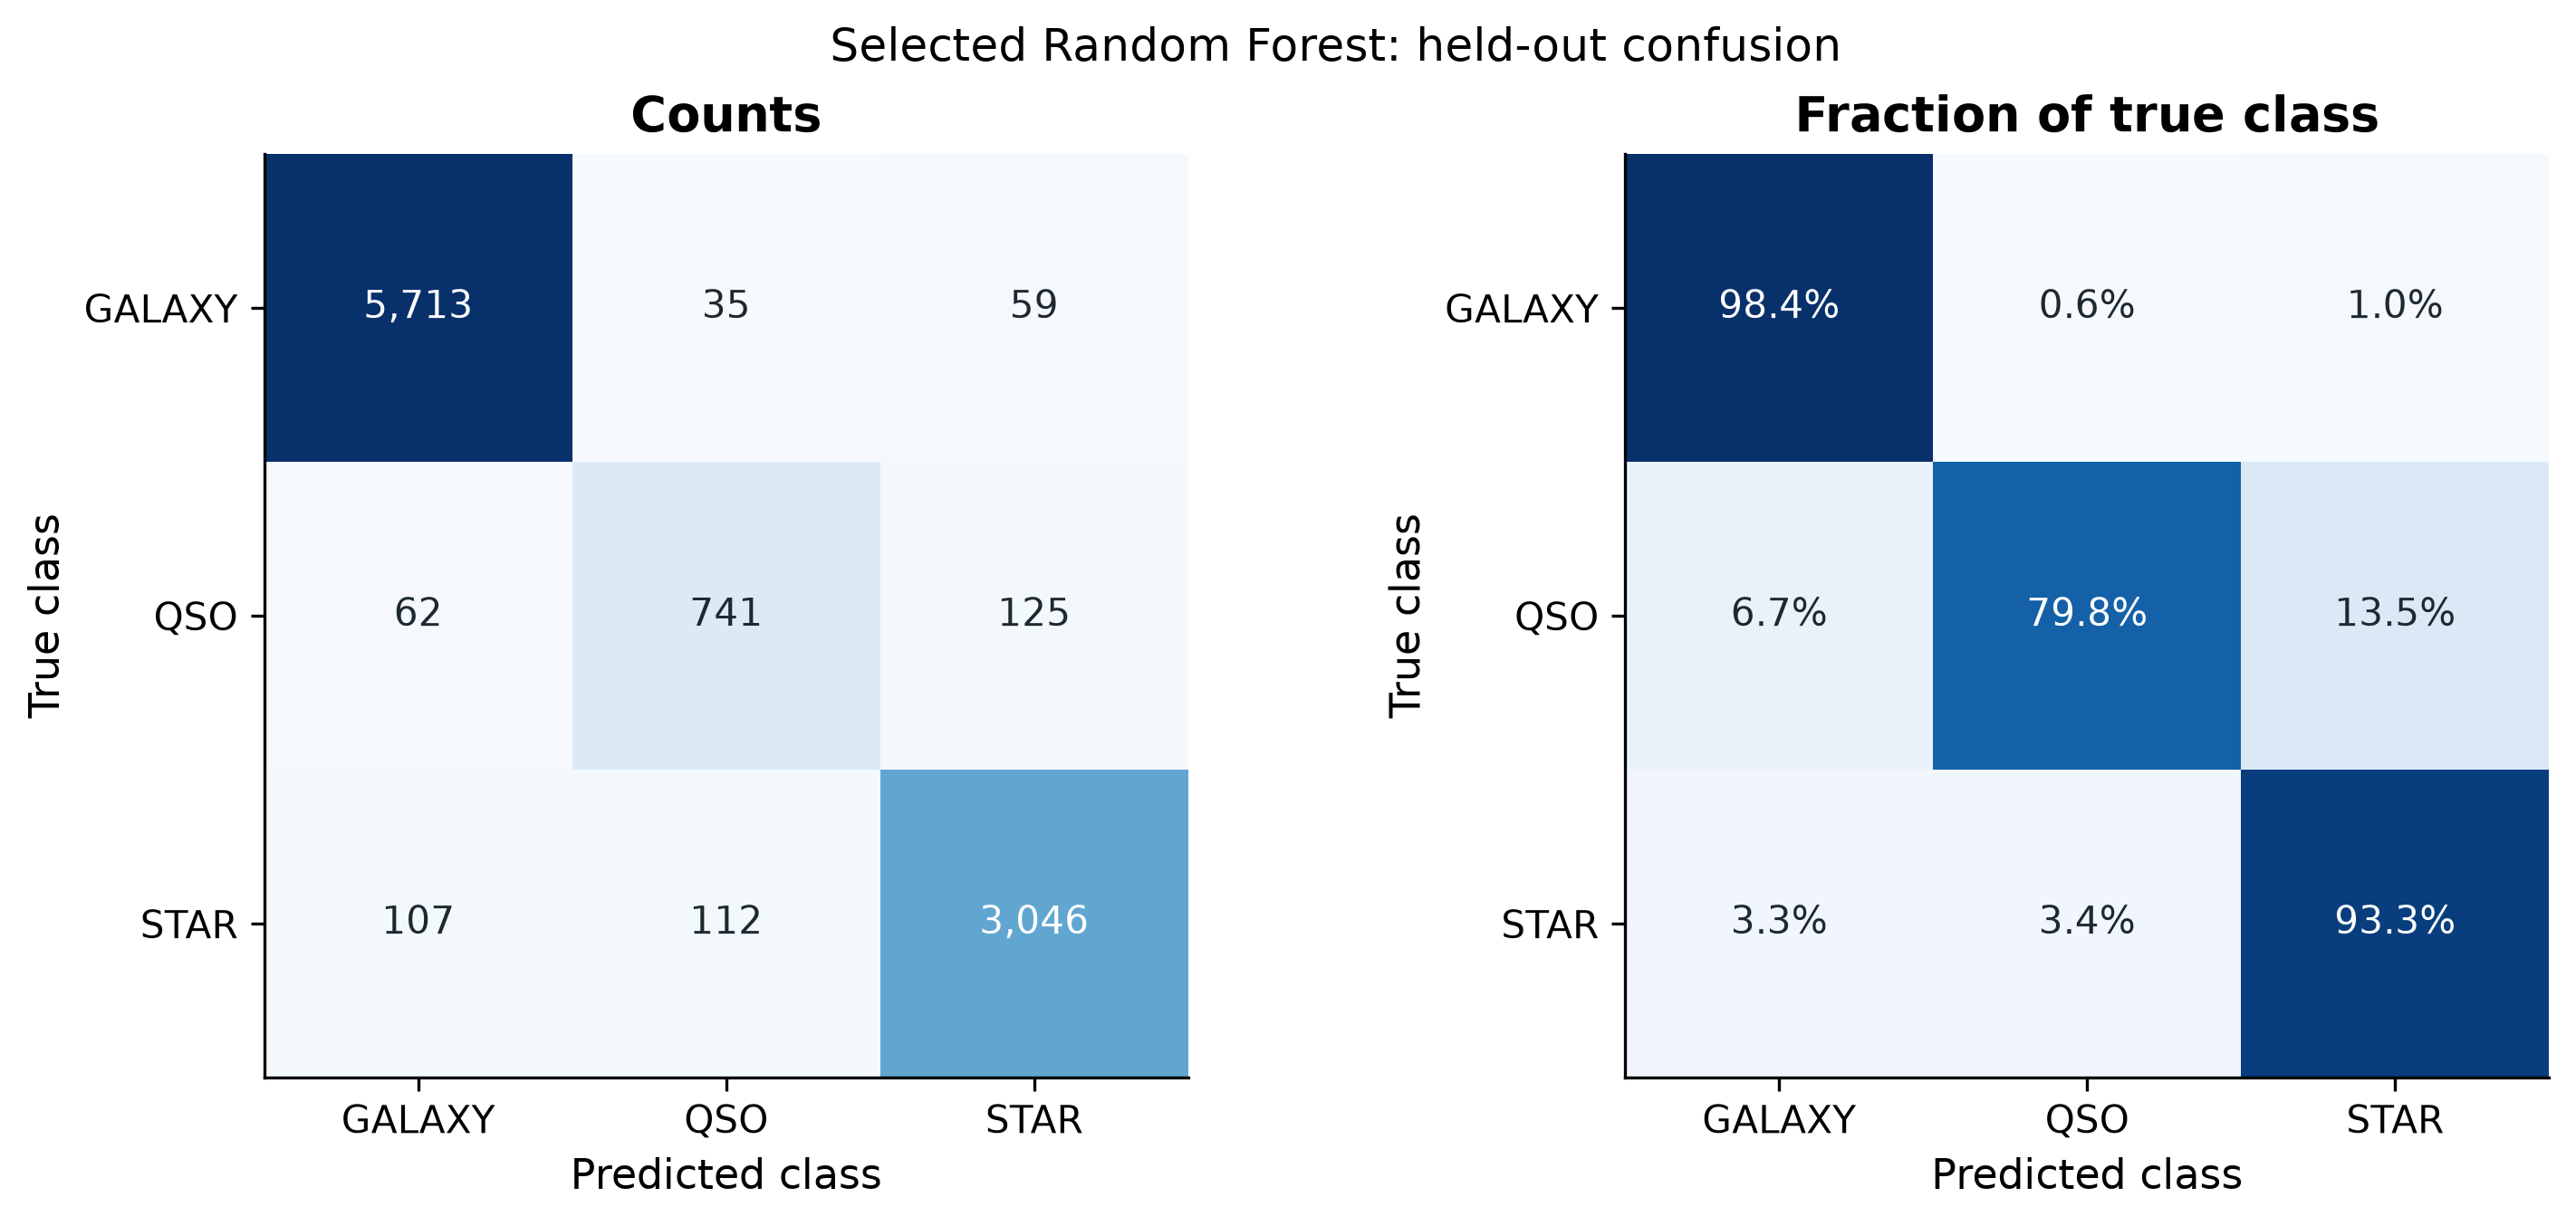
\includegraphics[width=0.87\textwidth]{confusion_matrix.png}
  \caption{Random Forest confusion matrix. Rows show the true class and
  columns show the prediction. The right panel divides each row by its total,
  making the classes easier to compare despite their different sizes.}
  \label{fig:confusion}
\end{figure}

\section{What explains the remaining errors?}
\subsection{Quasars are the hardest class}
Galaxy recall is 98.4\%, compared with 93.3\% for stars and 79.8\% for quasars.
The model classified 125 quasars as stars and 112 stars as quasars.
Together these account for 237 of the 500 errors (47.4\%).
The overlap in Figure~\ref{fig:colours} is consistent with this difficulty,
although a two-colour plot alone cannot establish the cause of the errors.

\subsection{Fainter objects are harder to classify}
The test objects were divided into five equally sized groups by their
$r$-band magnitude. Larger magnitudes mean fainter objects.
Accuracy falls from 98.85\% in the brightest group to 88.30\% in the faintest
group, a difference of 10.55 percentage points.

\begin{figure}[H]
  \centering
  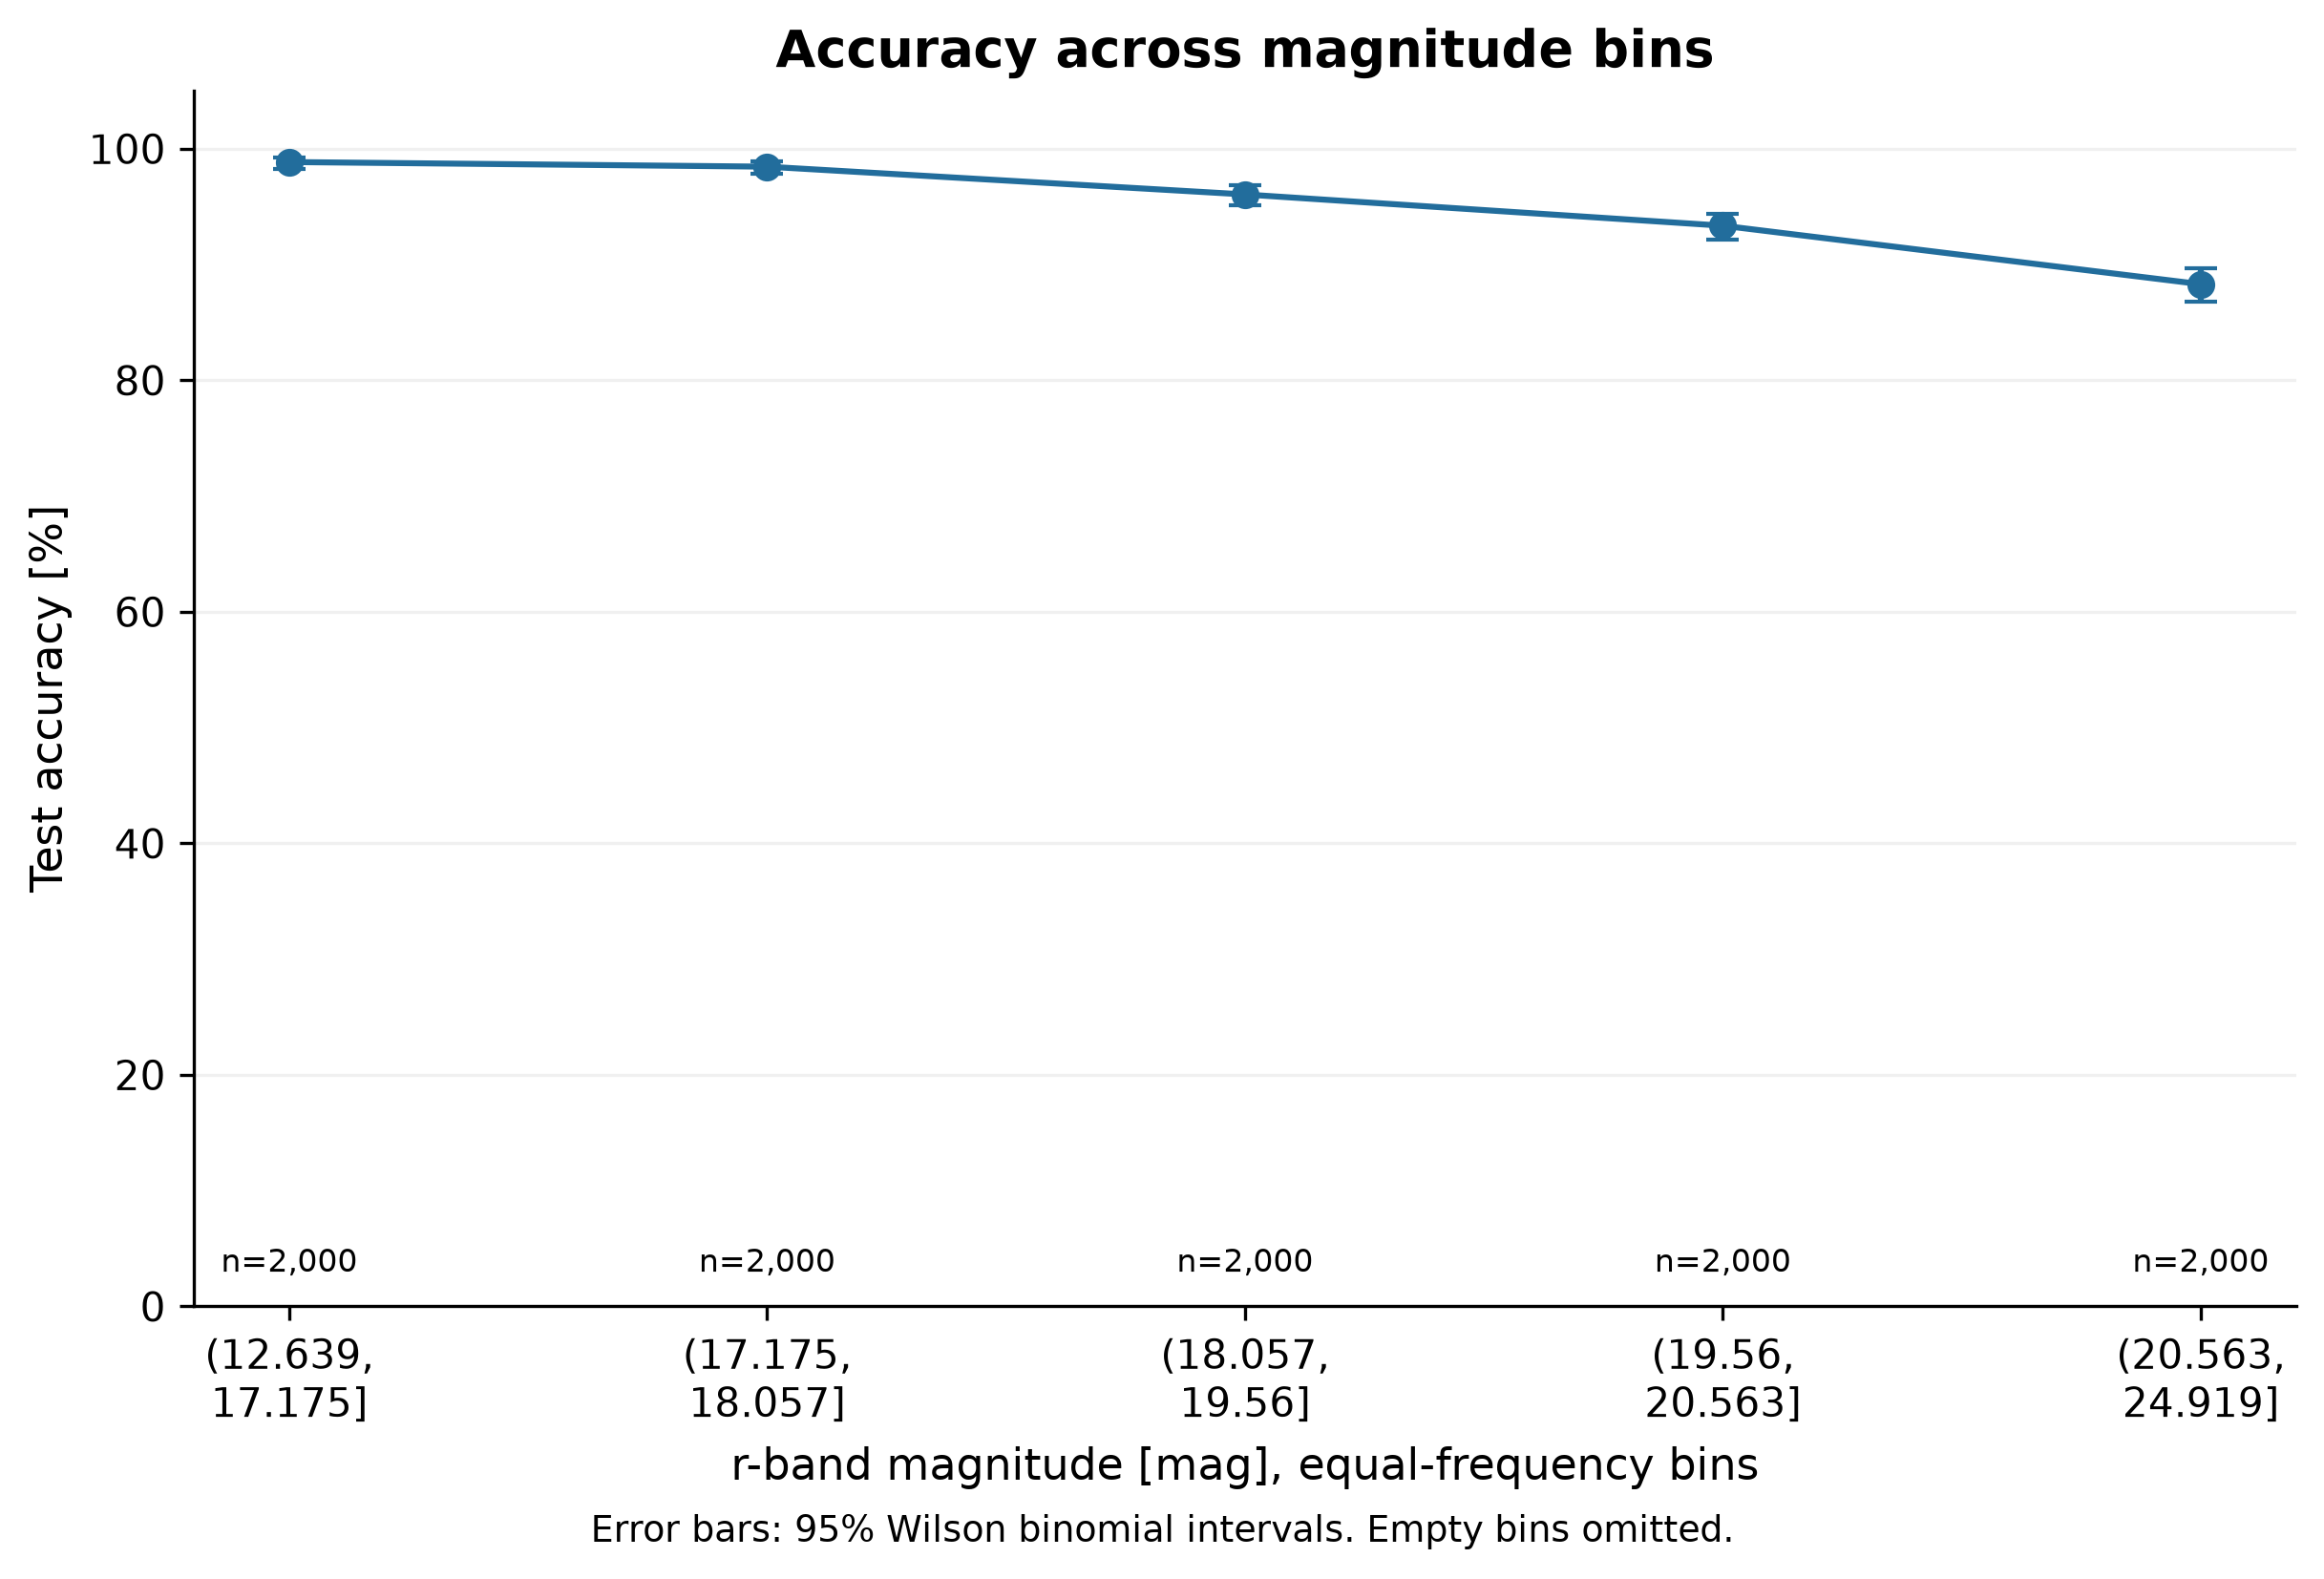
\includegraphics[width=0.73\textwidth]{accuracy_vs_magnitude.png}
  \caption{Random Forest accuracy across $r$-band magnitude groups, each
  containing 2,000 test objects. Error bars are 95\% Wilson binomial intervals,
  describing uncertainty from the finite number of objects in each group.}
  \label{fig:magnitude}
\end{figure}

Removing the five uncertainty features reduced accuracy by 1.89 percentage
points (Table~\ref{tab:models}), showing that they add predictive information.
Differences in brightness and class composition mean these associations
should not be interpreted as causal effects.

\section{Limitations and next steps}
This is a development study on one spectroscopically labelled sample.
Selection effects may limit how well the results apply to a wider catalogue.
The original acquisition query and \texttt{zWarning} column were not retained,
so the stated provenance and selection cuts cannot be fully checked.

Test results were also inspected during earlier development. Although tuning
now uses only training data, a fresh sample is needed for a fully independent
evaluation, with particular attention to faint objects and quasars.

\section{Conclusion}
The Random Forest achieved 95.00\% accuracy and a macro F1-score of 0.911
using 14 photometric features. The main weaknesses were quasar identification
and the classification of faint objects. The project established a repeatable
workflow for preparing data, comparing models and investigating their errors.

\begin{thebibliography}{9}\small
  \bibitem{sdss}
  Sloan Digital Sky Survey, \emph{Data Release 17}.
  \url{https://www.sdss4.org/dr17/}.
  \bibitem{sklearn}
  F. Pedregosa et al., \emph{Scikit-learn: Machine Learning in Python},
  \emph{Journal of Machine Learning Research}, 12, 2825--2830 (2011).
  \url{https://www.jmlr.org/papers/v12/pedregosa11a.html}.
\end{thebibliography}
\end{document}
